% Allow relative paths in included subfiles that are compiled separately
% See https://tex.stackexchange.com/questions/153312/
\providecommand{\main}{..}
\documentclass[\main/thesis.tex]{subfiles}

\begin{document}

\chapter{Background Information}
\chaptermark{background}
\label{chp:background}

In this chapter, I give a brief overview of the anatomy of a human heart.
Next, I describe the characteristics of a standard 12-lead \gls{ecg} and the notable waves in a \gls{ecg} signal.
I then give an overview of the \emph{PhysioNet/CinC 2020 Challenge} task/objective, provided dataset of \gls{ecg} records, and definitions for the diagnoses we are tasked to predict.

\section{Anatomy of a Heart Overview}

\begin{figure}[ht]
    \centering
    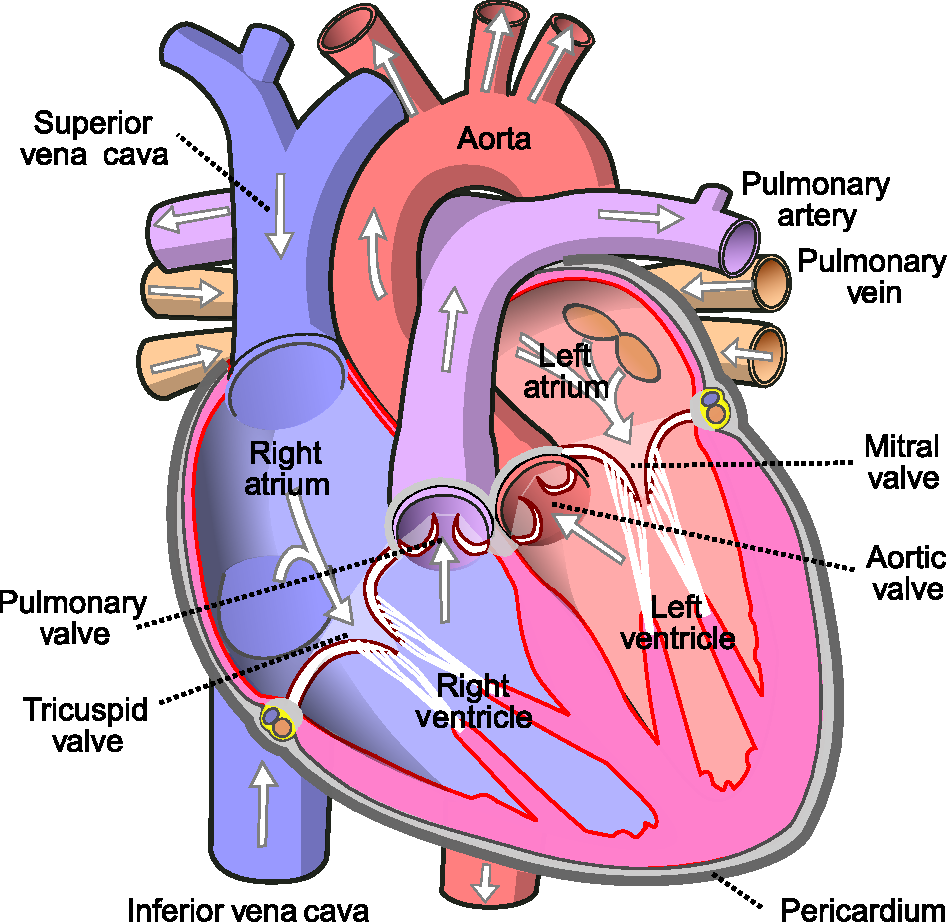
\includegraphics[width=8cm]{figure/Diagram_of_the_human_heart.pdf}
    \caption[Anterior, anatomical view of a human heart.]{Anterior, anatomical view of a human heart. The primary valves and chambers of the heart are annotated, with arrows indicating the direction of blood flow due to the contractions of the cardiac chambers. Image source: \href{https://upload.wikimedia.org/wikipedia/commons/e/e5/Diagram\_of\_the\_human\_heart\_\%28cropped\%29.svg?download}{\tt https://upload.wikimedia.org/wikipedia/commons/e/e5/Diagram\_of\_ the\_human\_heart\_\%28cropped\%29.svg?download}
    }
    \label{fig:heart_anatomy}
\end{figure}

A high level overview of the primary valves and chambers within the heart can be found in Figure~\ref{fig:heart_anatomy}.
TODO: heart anatomy, PQRST, axis

\section{Predicted Diagnoses}

\begin{description}
    \item[\gls{iavb}] TODO: Describe IAVB.
\end{description}

\gls{af}
\gls{afl}
\gls{brady}
\gls{crbbb}
\gls{irbbb}
\gls{lanfb}
\gls{lad}
\gls{lbbb}
\gls{lqrsv}
\gls{nsivcb}
\gls{pr}
\gls{pac}
\gls{pvc}
\gls{lpr}
\gls{lqt}
\gls{qab}
\gls{rad}
\gls{rbbb}
\gls{sa}
\gls{sb}
\gls{snr}
\gls{stach}
\gls{svpb}
\gls{tab}
\gls{tinv}
\gls{vpb}

% We plot an equation in figure \ref{fig:plot}.

% \begin{figure}
%     \centering
%     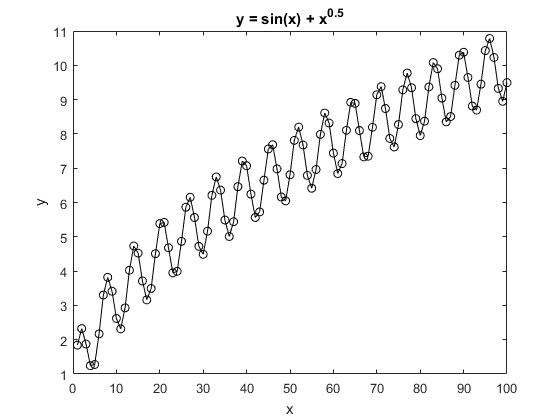
\includegraphics[keepaspectratio=true, width=0.9\textwidth]{\main/figure/plot}
%     \caption[A supporting figure] {A graph of $y = \sin(x) + \sqrt{x}$}
%     \label{fig:plot}
%     % Put the label *after* the caption, but inside the float
% \end{figure}

\end{document}